\providecommand{\main}{../..}
\documentclass[\main/notes.tex]{subfiles}

\begin{document}
	\setcounter{chapter}{10}
	\chapter{Systems Analysis}
		\section{An Overview of Systems Development}
			\begin{definition}{The Development Team}
				A team that consists of users, managers, systems development specialists, various support personnel and other stakeholders.

				Responsible for determining the objectives of the new information system, and delivering a system that meets these objectives.

				\begin{description}
					\item[Project] A planned collection of activities that achieves a goal, such as constructing a new manufacturing plant, or developing a new decision support system. Should have as defined starting and ending point.
					\item[Project Manager] A manager that is responsible for coordinating all people and resources needed to complete the project on time. Can be an IS person inside the organisation, or an external consultant. They need technical, business, and people skills. Usually responsible for controlling project quality, training personnel, facilitating communication, managing risks, and acquiring any necessary equipment.
					\item[Stakeholders] People who, either themselves or through the area of the organisation they represent, ultimately benefit from the systems development project.
					\item[Users] People who will interact with the system regularly. Can be employees, managers, or suppliers.
					\item[Systems Analyst] A professional who specialises in analysing and designing business systems.
						\begin{description}
							\item[Specialist Business Analysts] Experts in the business who try to identify ways in which new information systems can improve the current business processes.
						\end{description}
					\item[Programmer] Responsible for modifying or developing programs to satisfy user requirements. A programmer  takes plans from the systems analyst, and builds or modifies the necessary software.
					\item[Team Leader] Responsible for the development team. Can be from the IS department, a manager from the company, or a consultant. Needs both technical and people skills.
				\end{description}
			\end{definition}
			\subsection[Information Systems Planning]{Information Systems Planning and Aligning Organisation and IS Goals}
				\begin{definition}{Information Systems Planning}
					Translating strategic and organisational goals into systems development initiatives.

					Strategic goals must be finite, measurable, and tangible.
				\end{definition}
				\begin{sidenote}{The Steps of IS Planning}
					\begin{center}
						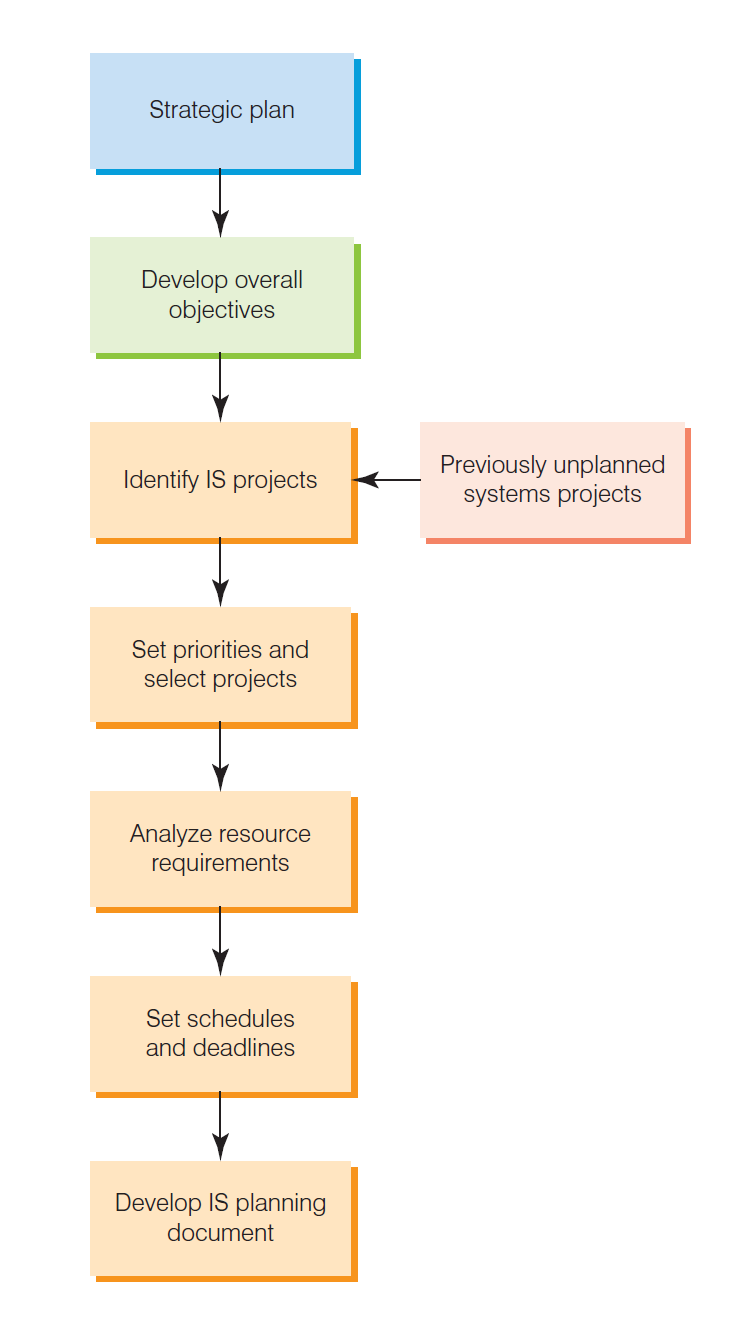
\includegraphics[width=0.6\textwidth]{chapter11/is_planning_steps.png}
					\end{center}
				\end{sidenote}
				\pagebreak
				\begin{definition}{Creative Analysis}
					The investigation of new approaches to existing problems. 

					Typically, inspired by people and events not directly related to the problem.
				\end{definition}
				\begin{definition}{Critical Analysis}
					The unbiased and careful questioning of whether system elements are related in the most effective ways.
					\begin{itemize}[nosep]
						\item Question statements and assumptions.
						\item Identify and resolve objectives and orientations that conflict.
					\end{itemize}
				\end{definition}
			\subsection{Establishing Objectives for Systems Development}
				\begin{sidenote}{Overall Objective}
					The overall objective of systems development is to achieve business goals, not technical goals, by delivering the right information to the right person at the right time.
				\end{sidenote}
				\begin{definition}{Critical Success Factors (CSFs)}
					Factors that are essential to the success of certain function areas of an organisation.
				\end{definition}
				\begin{definition}{Performance Objectives}
					The extent to which a system performs as desired.
					\begin{multicols}{2}
						\begin{itemize}[nosep]
							\item The quality or usefulness of the output
							\item The accuracy of the output
							\item The quality or usefulness of the format of the output
							\item The speed at which output is generated
							\item The scalability of the resulting system
							\item The degree to which business risk is reduced
						\end{itemize}
					\end{multicols}
				\end{definition}
				\begin{definition}{Cost Objectives}
					The costs associated with the system, should be minimised.
					\begin{multicols}{2}
						\begin{itemize}[nosep]
							\item Development costs
							\item Costs related to the uniqueness of the system application
							\item Fixed investments in hardware and related equipment
							\item Ongoing operating costs of the system
						\end{itemize}
					\end{multicols}
				\end{definition}
				Performance objectives and cost objectives should be balanced.

		\pagebreak
		\section{Systems Development Lifecycles (SDLC)}
			The systems development process is also called the \concept{systems development lifecycle (SDLC)}.
			\subsection{The Traditional Systems Development Lifecycle}
				\begin{definition}{Traditional Systems Development Lifecycle}
					Also known as the \concept{waterfall approach}.

					\begin{minipage}[t]{0.44\textwidth}
						\vspace{0pt}
						\begin{center}
							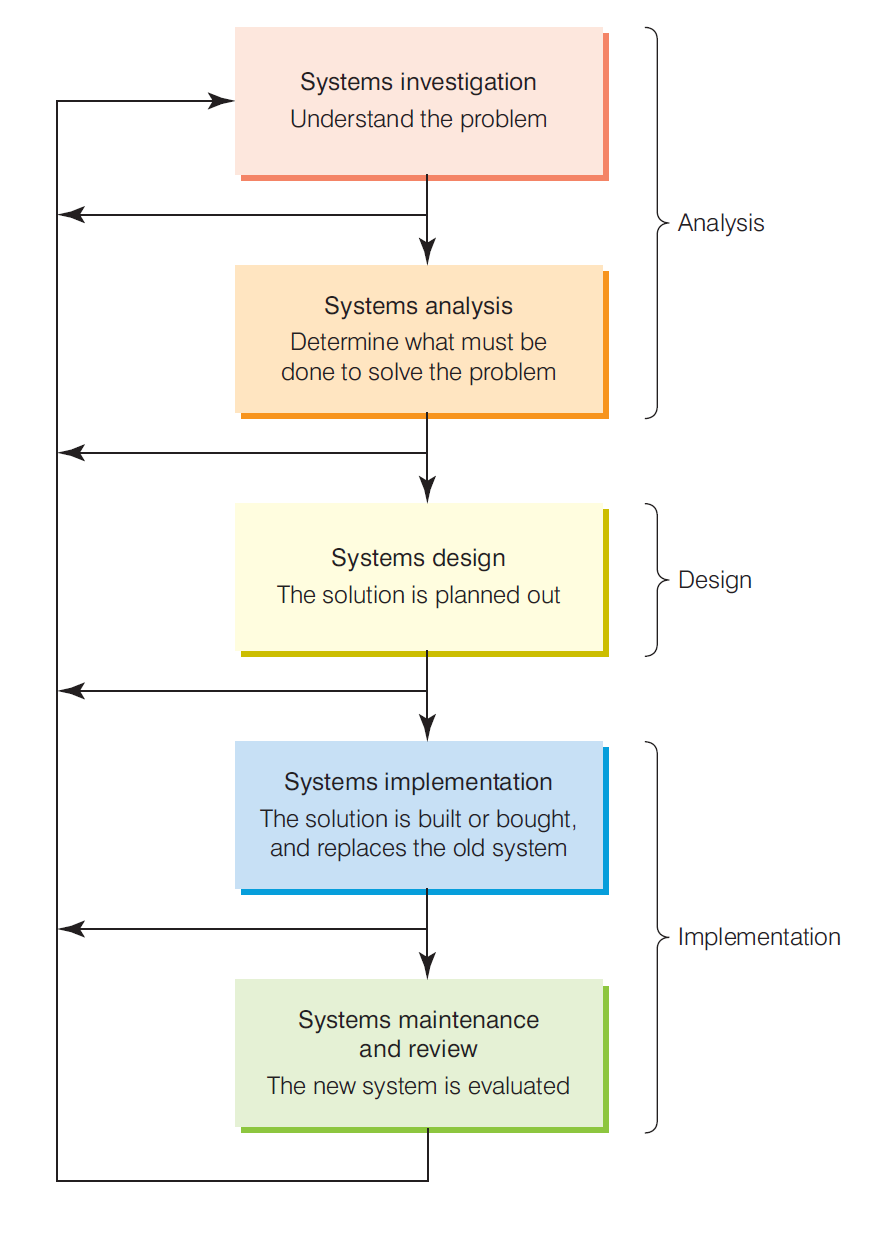
\includegraphics[width=0.95\linewidth]{chapter11/traditional_sdlc.png}
						\end{center}
					\end{minipage}
					\begin{minipage}[t]{0.55\textwidth}
						\vspace{0pt}
						\begin{description}
							\item[Systems Investigation] Problems and opportunities are identified and considered in light of the goals of the business. The result of this phase is a defined development project.
							\item[Systems Analysis] `What must the IS do to solve the problem?' Studies existing systems and work processes to identify strengths, weaknesses, and opportunities for improvement. The result of this phase is a list of requirements and priorities.
							\item[Systems Design] `How will the IS do what it must do to obtain the problem solution?' The result of this phase is a technical design that either describes the new system, or describes how existing systems will be modified.
							\item[Systems Implementation] Creating or buying the various system components detailed in the system design. The result of this phase is an installed, operational information system that meets the business needs for which it was developed.
							\item[Systems Maintenance and Review] Ensure that the system operates as intended, and modify the system so that it continues to meet changing business needs.
						\end{description}
					\end{minipage}
					\begin{center}
						\begin{tblr}{colspec={>{\raggedright}X|>{\raggedright}X}, row{1}={font=\bfseries}, row{even}={white}}
							Advantages & Disadvantages\\
							\midrule
							Formal review at the end of each phase allows maximum management control. & Users get a system that meets the needs as understood by the developers.\\
							Creates considerable system documentation. & Documentation expensive and time-consuming, and difficult to keep current.\\
							Formal docs ensure system requirements can be traced back to business needs. & User needs are unstated or misunderstood.\\
							Produces reviewable intermediate products. & Not easy for user to review intermediate products.
						\end{tblr}
					\end{center}
				\end{definition}
			\subsection{Prototyping}
				\begin{definition}{Prototyping}
					Also known as the \concept{evolutionary lifecycle}. Takes an iterative approach to systems development. During each iteration, requirements and alternative solutions to the problem are identified and analysed, new solutions are designed, and a portion of the system is implemented.
					\begin{description}
						\item[Operational Prototype] A prototype that has functionality -- it does something towards solving the problem. May accept input, partially process it, and output the results.
						\item[Non-operational Prototype] A mock-up or model. Includes input specifications and formats. Can be developed much faster than an operational prototype.
					\end{description}
					\begin{center}
						\begin{tblr}{colspec={>{\raggedright}X|>{\raggedright}X}, row{1}={font=\bfseries}, row{even}={white}}
							Advantages & Disadvantages\\
							\midrule
							Users can try the system and provide constructive feedback during development. & The final solution might be only incrementally better than the initial solution.\\
							An operational prototype can be produced in weeks & Formal end-of-phase reviews might not occur. It is difficult to contain the scope of the prototype -- the project never seems to end.\\
							As solutions emerge, users become more positive about the process and the results & System documentation is often absent or incomplete.\\
							Enables early detection of errors and omissions. & System backup and recovery, performance, and security issues can be overlooked in the haste to develop a prototype.
						\end{tblr}
					\end{center}
				\end{definition}
			\subsection{Other Systems Development Approaches}
				\begin{definition}{Rapid Application Development (RAD)}
					A systems development approach that employs tools, techniques, and methodologies designed to speed application development.

					Reduces paper-based documentation, automatically generates program source code, and facilitates user participation in design and development activities.
					\begin{description}
						\item[Joint Application Development (JAD)] Used for data collection and requirements analysis. Involves group meetings in which users, stakeholders, and IS professionals work together to analyse existing systems, propose possible solutions, and define the requirements for a new or modified system. Often uses \concept{group support systems (GSS)} software to foster positive group interactions.
					\end{description}
					Generally, RAD is better suited for DSS's and MIS's, and less well suited for TPS's.
				\end{definition}
				\pagebreak
				\begin{sidenote}{Advantages and Disadvantages of RAD}
					\begin{center}
						\begin{tblr}{colspec={>{\raggedright}X|>{\raggedright}X}, row{1}={font=\bfseries}, row{even}={white}}
							Advantages & Disadvantages\\
							\midrule
							Puts an application into production sooner than any other approach & Can burn out systems developers and other project participants\\
							Documentation is produced as a by-product of completing project tasks & Requires systems analysts and users to be skilled in RAD systems development tools and RAD techniques.\\
							Forces teamwork and lots of interaction between users and stakeholders & Requires a larger percentage of stakeholders' and users' time than other approaches.
						\end{tblr}
					\end{center}
				\end{sidenote}
				\begin{definition}{Agile Development}
					Allows the systems to change as they are being developed. Requires frequent face-to-face meetings with the systems developers and users as they modify, refine, and test how the system meets users' needs, and what its capabilities are.
					\begin{description}
						\item[Extreme Programming (XP)] Uses pairs of programmers who work together to design, test, and code parts of the systems they develop.
					\end{description}
				\end{definition}
			\subsection{The End-User Systems Development Lifecycle}
				\begin{definition}{End-User Systems Development Lifecycle}
					Any systems development project in which business managers and users assume the primary effort.
				\end{definition}
			\subsection{Outsourcing and On-Demand Computing}
				\begin{sidenote}{Outsourcing}
					A good idea if:
					\begin{itemize}[nosep]
						\item A company believes it can cut costs.
						\item A firm has limited opportunity to distinguish itself competitively through a particular IS operation or application.
						\item Uninterrupted IS service is not crucial.
						\item Outsourcing does not strip the company of technical know-how required for future IS innovation.
						\item The firm's existing IS capabilities are limited, ineffective, or technically inferior.
						\item A firm is downsizing.
							\begin{description}
								\item[Downsizing] Reducing the number of employees or managers, equipment and systems, and even functions and departments. 
							\end{description}
					\end{itemize}
				\end{sidenote}
			\subsection{Genetic Programming}
				\begin{definition}{Genetic Programming}
					An approach to creating computer code based on natural selection. Initially random code evolves through numerous iterations to become a program that solves a set problem.
				\end{definition}

	\vbox{\rulechapterend}
\end{document}